\documentclass[12pt]{article}
\usepackage[utf8]{inputenc}
\usepackage{listings}
\usepackage{inconsolata}
\usepackage[usenames,dvipsnames]{xcolor}
\usepackage[margin=1in]{geometry}
\usepackage{algorithmicx}
\usepackage{algpseudocode}
\usepackage{amsmath}
\usepackage{tikz}
\usepackage{mathtools}
\usepackage{proof}
\usepackage{graphicx}

\usetikzlibrary{positioning}

\algrenewcommand{\algorithmicforall}{\textbf{for each}}

\newcommand*{\lineref}[1]{$\langle$line #1$\rangle$}
\newcommand*{\objref}[1]{$\langle$object \texttt{#1}$\rangle$}
\newcommand*{\voidref}[1]{\texttt{void}}
\newcommand*{\so}{\textit{so}}
\newcommand*{\Int}{\mathrm{Int}}

\lstdefinelanguage{Cool}{
    morekeywords = {if,fi,pool,loop,while,else,class,inherits,case,in,of,esac,let,new,try,catch,yrt,throw},
    morekeywords = [2]{Int,Object,Value,MulOp,AddOp,Stack,Main,IO,SELF_TYPE},
    morecomment=[l]{--},
    morecomment=[n]{(*}{*)},
    morestring=[b]{"},
    literate={<-}{$\gets{}$}{2}{<=}{$\le{}$}{2}{=>}{$\Rightarrow{}$}{2},
}
\lstdefinestyle{mystyle}{
    numbers=left,numberstyle=\tiny,numbersep=10pt,
    commentstyle=\color{gray},
    keywordstyle=\bfseries,
    keywordstyle={[2]\color{BlueViolet}},
    stringstyle=\color{Mahogany},
    numberstyle=\color{darkgray},
}
\lstset{
    basicstyle=\ttfamily\small,
    tabsize=2,
    style=mystyle,
}

\title{CS143 Written Assignment 4}
\author{Your Name -- SUNet ID}
\date{Due: June 4th, 2024 EOD}

\begin{document}
\maketitle

\begin{enumerate}

\item
    \begin{enumerate}

        \item
            \texttt{Value}:

            \begin{tabular}{ll}  % the sample dispatch table for Stack
                \hline
                Address & Line Number (Method) \\
                \hline
                0x8000 & \lineref{17} (\texttt{get}) \\
                0x8008 & \lineref{18} (\texttt{pop}) \\
                0x8010 & \lineref{19} (\texttt{set}) \\
                0x8018 & \lineref{20} (\texttt{push}) \\
                \hline
            \end{tabular}

            \vspace{1em}\texttt{MulOp}:

            \begin{tabular}{ll}
                \hline
                Address & Line Number (Method) \\
                \hline
                0x8000 & \lineref{17} (\texttt{get}) \\
                0x8008 & \lineref{18} (\texttt{pop}) \\
                0x8010 & \lineref{19} (\texttt{set}) \\
                0x8018 & \lineref{20} (\texttt{push}) \\
                \hline
            \end{tabular}

            \vspace{1em}\texttt{AddOp}:

            \begin{tabular}{ll}
                \hline
                Address & Line Number (Method) \\
                \hline
                0x8000 & \lineref{17} (\texttt{get}) \\
                0x8008 & \lineref{18} (\texttt{pop}) \\
                0x8010 & \lineref{19} (\texttt{set}) \\
                0x8018 & \lineref{20} (\texttt{push}) \\
                \hline
            \end{tabular}

        \clearpage
        \item Heap layout:

        \begin{tabular}{lll}  % sample heap layout
            \hline
            Address & Value & Meaning \\
            \hline
            \objref{Main} + 0x0000 & 5 & (class tag) \\
            \objref{Main} + 0x0008 & 4 & (object size) \\
            \objref{Main} + 0x0010 & 0x8800 & (dispatch ptr) \\
            \objref{Main} + 0x0018 & \voidref{} & (\texttt{stack}) \\
            \hline
        \end{tabular}

        \clearpage
        \item Stack layout:

        \begin{tabular}{lll}  % sample stack layout
            \hline
            Address & Value & Meaning \\
            \hline
            0x7777fff8 & 0x7ffffff8 & (saved frame pointer) \\
            0x7777fff0 & \objref{Main} & (argument 0 of \texttt{main}) \\
            0x7777ffe8 & 0x2000 & (return address of \texttt{main}) \\
            0x7777ffe0 & \objref{IO} & (local variable \texttt{io}) \\
            0x7777ffd8 & 5 & (local variable \texttt{num}) \\
            0x7777ffd0 & 0x7777ffe8 & (saved frame pointer) \\
            0x7777ffc8 & 5 & (argument 1 of \texttt{init}) \\
            0x7777ffc0 & \objref{Main} & (argument 0 of \texttt{init}) \\
            0x7777ffb8 & \lineref{53} & (return address of \texttt{init}) \\
            \hline
        \end{tabular}

    \end{enumerate}

    \clearpage
    \item \begin{enumerate}
        \item % for reference, here is the [Neg] rule from the Cool manual
            \[ \infer[\text{[Neg]}]{
                \so, S_1, E \vdash \mathord{\sim} e_1 \mapsto v_1, S_2
            }{
                \so, S_1, E \vdash e_1 \mapsto \Int(i_1), S_2 &
                v_1 = \Int(-i_1)
            } \]

        \clearpage
        \item % reference proof tree
        \[ % you may find it necessary to decrease the font size:
        % \scriptsize
        \infer[\text{[Arith]}]{
            \vdash 2 * \mathord{\sim}1 \mapsto \Int(-2), S
        }{
            \infer[\text{[Int]}]{\vdash 2 \mapsto \Int(2), S}{} &
            \infer[\text{[Neg]}]{\vdash \mathord{\sim}1 \mapsto \Int(-1), S}{
                \infer[\text{[Int]}]{\vdash 1 \mapsto \Int(1), S}{}
            }
        } \]

        \clearpage
        \item Simple Simplicio...

        \begin{lstlisting}[language=Cool]
class Main {
    main() : Int {
        1 + 1
    };
};
        \end{lstlisting}
    \end{enumerate}

    \clearpage
    \item
    \begin{enumerate}
        \item Optimized CFG: % (here's the original CFG)

        \begin{center}
        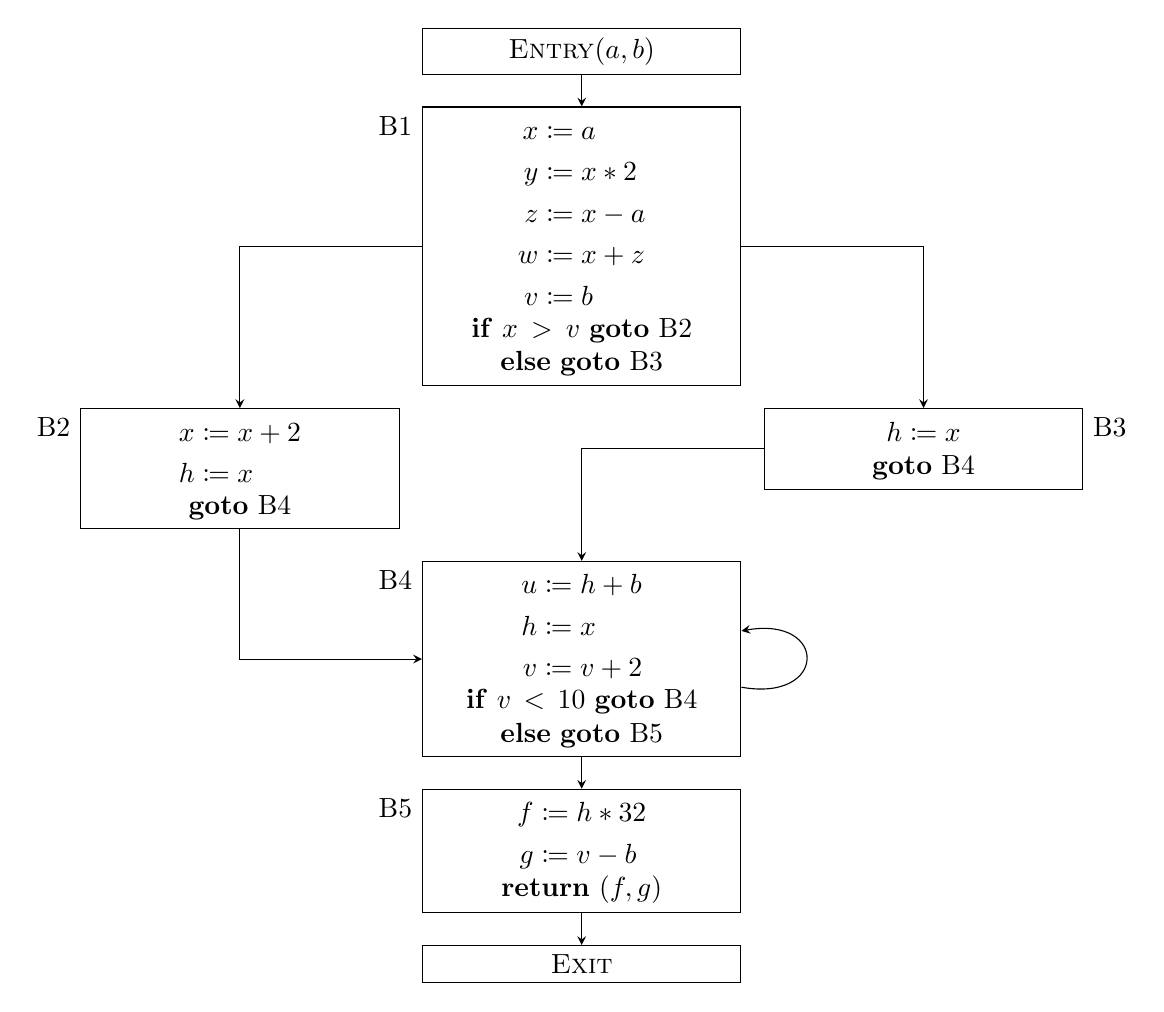
\begin{tikzpicture}[bb/.style={text width=1.5in, draw, align=center}, node distance=0.4cm]
            \node[bb] (entry) {\textsc{Entry}($a, b$)};
            \node[bb,below=of entry] (b1) {$\begin{aligned}
                x &\coloneqq a \\
                y &\coloneqq x * 2 \\
                z &\coloneqq x - a \\
                w &\coloneqq x + z \\
                v &\coloneqq b \\
            \end{aligned}$ \\
            \textbf{if} $x > v$ \textbf{goto} B2 \\
            \textbf{else goto} B3};
            \node[bb,below left=of b1] (b2) {$\begin{aligned}
                x &\coloneqq x + 2 \\
                h &\coloneqq x \\
            \end{aligned}$ \\
            \textbf{goto} B4};
            \node[bb,below right=of b1] (b3) {$\begin{aligned}
                h &\coloneqq x \\
            \end{aligned}$ \\
            \textbf{goto} B4};
            \node[bb,below=of {b1.south |- b2.south}] (b4) {$\begin{aligned}
                u &\coloneqq h + b \\
                h &\coloneqq x \\
                v &\coloneqq v + 2 \\
            \end{aligned}$ \\
            \textbf{if} $v < 10$ \textbf{goto} B4 \\
            \textbf{else goto} B5};
            \node[bb,below=of b4] (b5) {$\begin{aligned}
                f &\coloneqq h * 32 \\
                g &\coloneqq v - b \\
            \end{aligned}$ \\
            \textbf{return} $(f, g)$};
            \node[bb,below=of b5] (exit) {\textsc{Exit}};
            \node[left=0pt of b1.north west, anchor=north east] {B1};
            \node[left=0pt of b2.north west, anchor=north east] {B2};
            \node[right=0pt of b3.north east, anchor=north west] {B3};
            \node[left=0pt of b4.north west, anchor=north east] {B4};
            \node[left=0pt of b5.north west, anchor=north east] {B5};
            \draw[->,>=stealth] (entry) -- (b1);
            \draw[->,>=stealth] (b1.west) -| (b2.north);
            \draw[->,>=stealth] (b1.east) -| (b3.north);
            \draw[->,>=stealth] (b2.south) |- (b4.west);
            \draw[->,>=stealth] (b3.west) -| (b4.north);
            \draw[->,>=stealth] (b4) edge[loop right,in=10,out=-10,looseness=4] (b4);
            \draw[->,>=stealth] (b4) -- (b5);
            \draw[->,>=stealth] (b5) -- (exit);
        \end{tikzpicture}
        \end{center}

        \clearpage
        \item Optimized CFG: % (here's the original CFG)

        \begin{center}
        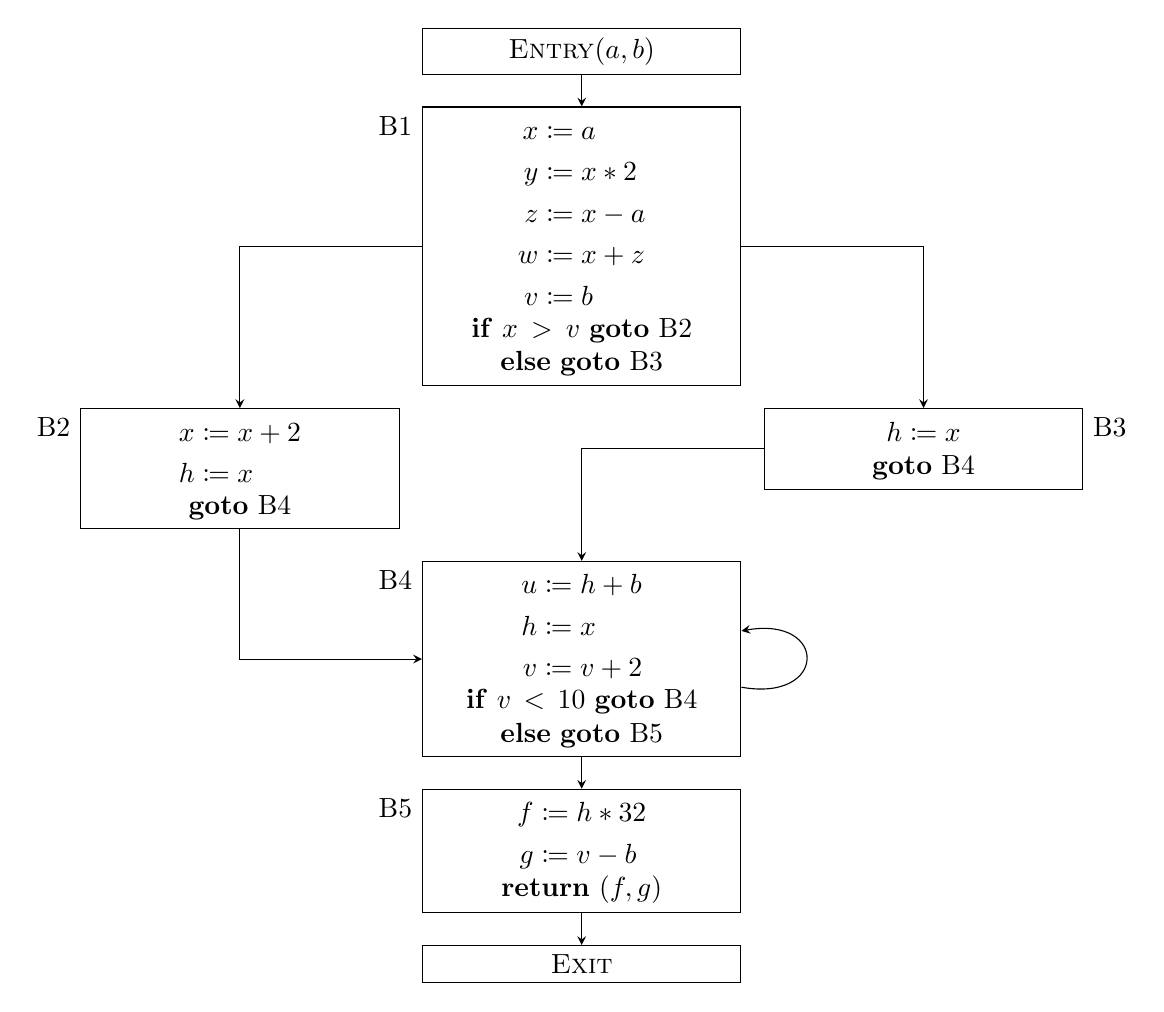
\begin{tikzpicture}[bb/.style={text width=1.5in, draw, align=center}, node distance=0.4cm]
            \node[bb] (entry) {\textsc{Entry}($a, b$)};
            \node[bb,below=of entry] (b1) {$\begin{aligned}
                x &\coloneqq a \\
                y &\coloneqq x * 2 \\
                z &\coloneqq x - a \\
                w &\coloneqq x + z \\
                v &\coloneqq b \\
            \end{aligned}$ \\
            \textbf{if} $x > v$ \textbf{goto} B2 \\
            \textbf{else goto} B3};
            \node[bb,below left=of b1] (b2) {$\begin{aligned}
                x &\coloneqq x + 2 \\
                h &\coloneqq x \\
            \end{aligned}$ \\
            \textbf{goto} B4};
            \node[bb,below right=of b1] (b3) {$\begin{aligned}
                h &\coloneqq x \\
            \end{aligned}$ \\
            \textbf{goto} B4};
            \node[bb,below=of {b1.south |- b2.south}] (b4) {$\begin{aligned}
                u &\coloneqq h + b \\
                h &\coloneqq x \\
                v &\coloneqq v + 2 \\
            \end{aligned}$ \\
            \textbf{if} $v < 10$ \textbf{goto} B4 \\
            \textbf{else goto} B5};
            \node[bb,below=of b4] (b5) {$\begin{aligned}
                f &\coloneqq h * 32 \\
                g &\coloneqq v - b \\
            \end{aligned}$ \\
            \textbf{return} $(f, g)$};
            \node[bb,below=of b5] (exit) {\textsc{Exit}};
            \node[left=0pt of b1.north west, anchor=north east] {B1};
            \node[left=0pt of b2.north west, anchor=north east] {B2};
            \node[right=0pt of b3.north east, anchor=north west] {B3};
            \node[left=0pt of b4.north west, anchor=north east] {B4};
            \node[left=0pt of b5.north west, anchor=north east] {B5};
            \draw[->,>=stealth] (entry) -- (b1);
            \draw[->,>=stealth] (b1.west) -| (b2.north);
            \draw[->,>=stealth] (b1.east) -| (b3.north);
            \draw[->,>=stealth] (b2.south) |- (b4.west);
            \draw[->,>=stealth] (b3.west) -| (b4.north);
            \draw[->,>=stealth] (b4) edge[loop right,in=10,out=-10,looseness=4] (b4);
            \draw[->,>=stealth] (b4) -- (b5);
            \draw[->,>=stealth] (b5) -- (exit);
        \end{tikzpicture}
        \end{center}

    \end{enumerate}

    \clearpage
    \item

    \begin{enumerate}
        \item Live variables:

        \begin{center}
        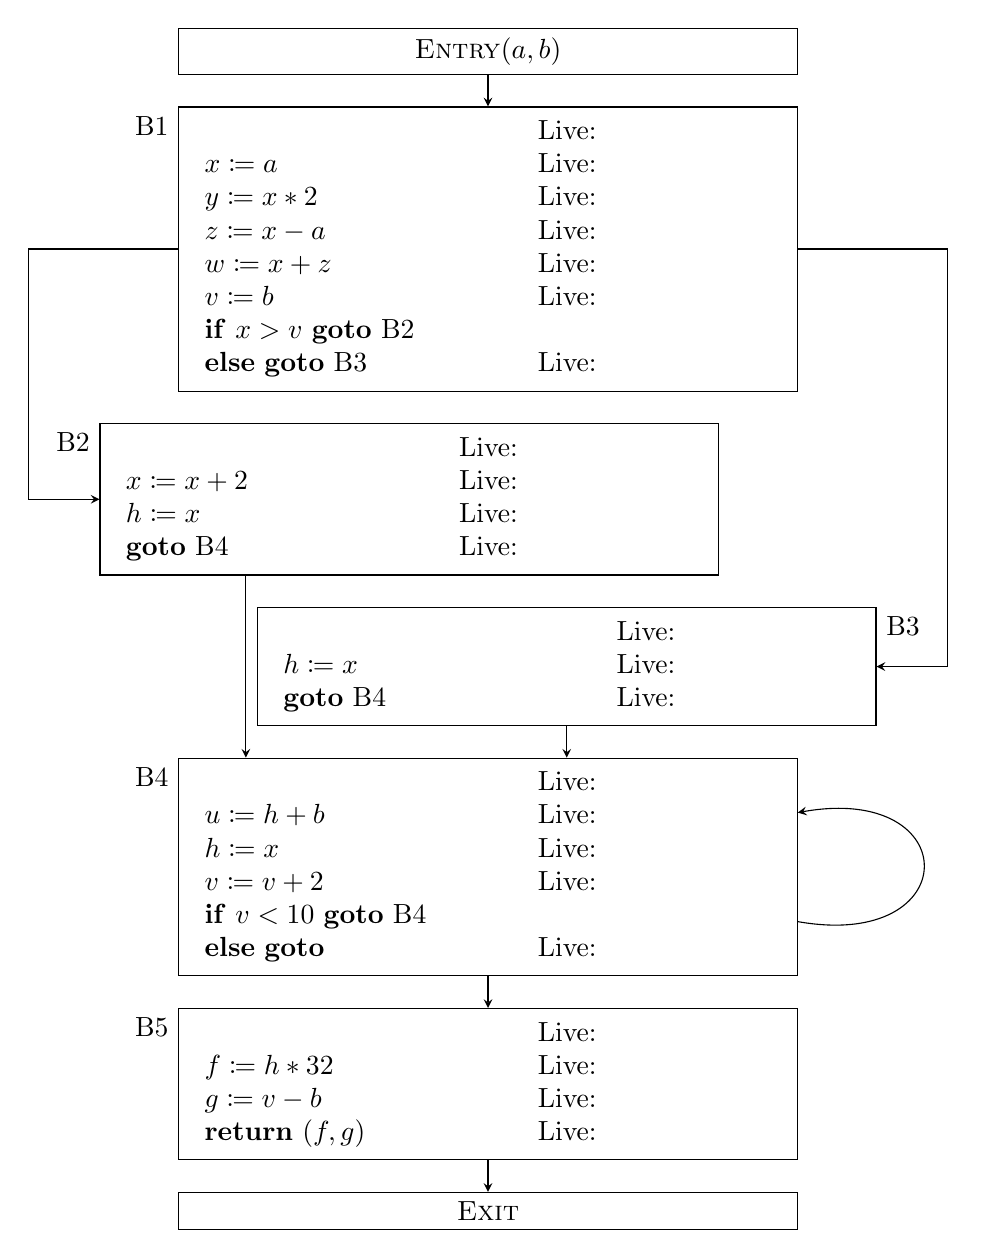
\begin{tikzpicture}[bb/.style={text width=3in, draw}, node distance=0.4cm]
            \node[bb,align=center] (entry) {\textsc{Entry}($a, b$)};
            \node[bb,below=of entry] (b1) {\begin{tabular}{p{1.5in}l}
                                                                   & Live: \\
                $x \coloneqq a$                                    & Live: \\
                $y \coloneqq x * 2$                                & Live: \\
                $z \coloneqq x - a$                                & Live: \\
                $w \coloneqq x + z$                                & Live: \\
                $v \coloneqq b$                                    & Live: \\
                \textbf{if} $x > v$ \textbf{goto} B2 \\
                \textbf{else goto} B3                              & Live: \\
            \end{tabular}};
            \node[bb,below left=0.4cm and 1cm of b1.south,anchor=north] (b2) {\begin{tabular}{p{1.5in}l}
                                                                   & Live: \\
                $x \coloneqq x + 2$                                & Live: \\
                $h \coloneqq x$                                    & Live: \\
                \textbf{goto} B4                                   & Live:
            \end{tabular}};
            \node[bb,below right=0.4cm and 1cm of b1.south |- b2.south,anchor=north] (b3) {\begin{tabular}{p{1.5in}l}
                                                                   & Live: \\
                $h \coloneqq x$                                    & Live: \\
                \textbf{goto} B4                                   & Live:
            \end{tabular}};
            \node[bb,below=of {b1.south |- b3.south}] (b4) {\begin{tabular}{p{1.5in}l}
                                                                   & Live: \\
                $u \coloneqq h + b$                                & Live: \\
                $h \coloneqq x$                                    & Live: \\
                $v \coloneqq v + 2$                                & Live: \\
                \textbf{if} $v < 10$ \textbf{goto} B4 \\
                \textbf{else goto}                                 & Live:
            \end{tabular}};
            \node[bb,below=of b4] (b5) {\begin{tabular}{p{1.5in}l}
                                                                   & Live: \\
                $f \coloneqq h * 32$                               & Live: \\
                $g \coloneqq v - b$                                & Live: \\
                \textbf{return} $(f, g)$                           & Live:
            \end{tabular}};
            \node[bb,below=of b5,align=center] (exit) {\textsc{Exit}};
            \node[left=0pt of b1.north west, anchor=north east] {B1};
            \node[left=0pt of b2.north west, anchor=north east] {B2};
            \node[right=0pt of b3.north east, anchor=north west] {B3};
            \node[left=0pt of b4.north west, anchor=north east] {B4};
            \node[left=0pt of b5.north west, anchor=north east] {B5};
            \draw[->,>=stealth] (entry) -- (b1);
            \draw[->,>=stealth] (b1.west) -- +(-0.75in,0) |- (b2.west);
            \draw[->,>=stealth] (b1.east) -- +( 0.75in,0) |- (b3.east);
            \draw[->,>=stealth] (b2.205) -- (b4.north -| b2.205);
            \draw[->,>=stealth] (b3.south) -- (b4.north -| b3.south);
            \draw[->,>=stealth] (b4) edge[loop right,in=10,out=-10,looseness=4] (b4);
            \draw[->,>=stealth] (b4) -- (b5);
            \draw[->,>=stealth] (b5) -- (exit);
        \end{tikzpicture}
        \end{center}

        \clearpage
        \item Interference graph:

        \begin{centering} % sample interference graph
        \begin{tikzpicture}[every node/.style={minimum width=3em, circle, draw}]
            % if you aren't already familiar with TikZ
            % I would recommend using another tool
            \node (a) at (0:2cm) {$a$};
            \node (b) at (120:2cm) {$b$};
            \node (c) at (240:2cm) {$c$};
            \node (d) at (0:5cm) {$d$};
            \draw (a) -- (b);
            \draw (b) -- (c);
            \draw (a) -- (c);
            \draw (a) -- (d);
        \end{tikzpicture}
        \end{centering}

        Edge list:

        \begin{verbatim}
a - b;
b - c;
a - c;
a - d;
\end{verbatim}

        % here's how to include an image
        % \includegraphics[width=0.5\textwidth]{colored_graph.png}

        \clearpage
        \item Coloring:

        \begin{centering} % sample interference graph, colored
        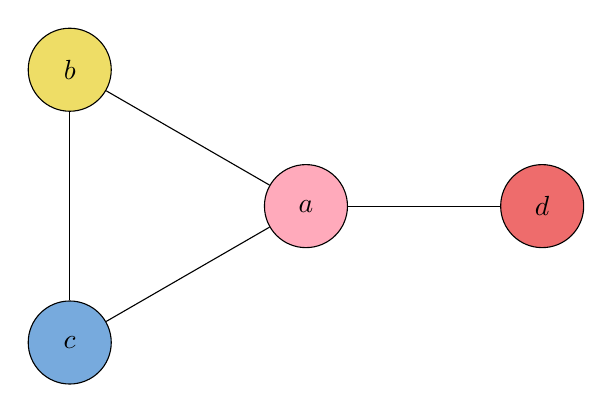
\begin{tikzpicture}[every node/.style={minimum width=3em, circle, draw}]
            % I've provided some colors to use as color1-9
            % they should be relatively colorblind friendly
            \definecolor{color1}{HTML}{FFAABB}
            \definecolor{color2}{HTML}{EEDD66}
            \definecolor{color3}{HTML}{77AADD}
            \definecolor{color4}{HTML}{EE6C6C}
            \definecolor{color5}{HTML}{99DDFF}
            \definecolor{color6}{HTML}{44BB99}
            \definecolor{color7}{HTML}{BBCC33}
            \definecolor{color8}{HTML}{AAAA00}
            \definecolor{color9}{HTML}{DDDDDD}
            \node[fill=color1] (a) at (0:2cm) {$a$};
            \node[fill=color2] (b) at (120:2cm) {$b$};
            \node[fill=color3] (c) at (240:2cm) {$c$};
            \node[fill=color4] (d) at (0:5cm) {$d$};
            \draw (a) -- (b);
            \draw (b) -- (c);
            \draw (a) -- (c);
            \draw (a) -- (d);
        \end{tikzpicture}
        \end{centering}

        Here are 9 colors chosen to be reasonably distinct for
        color-blind and non-color-blind vision:

        \begin{centering} % sample interference graph, colored
        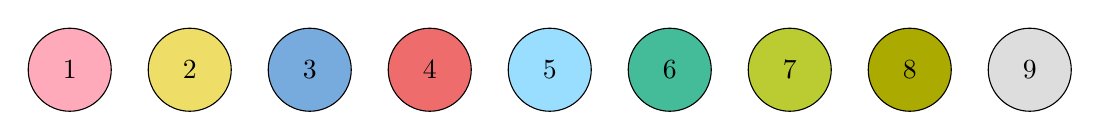
\begin{tikzpicture}[every node/.style={minimum width=3em, circle, draw},x=0.6in]
            % I've provided some colors to use as color1-9
            % they should be relatively colorblind friendly
            \definecolor{color1}{HTML}{FFAABB}
            \definecolor{color2}{HTML}{EEDD66}
            \definecolor{color3}{HTML}{77AADD}
            \definecolor{color4}{HTML}{EE6C6C}
            \definecolor{color5}{HTML}{99DDFF}
            \definecolor{color6}{HTML}{44BB99}
            \definecolor{color7}{HTML}{BBCC33}
            \definecolor{color8}{HTML}{AAAA00}
            \definecolor{color9}{HTML}{DDDDDD}
            \node[fill=color1] (a) at (0,0) {1};
            \node[fill=color2] (b) at (1,0) {2};
            \node[fill=color3] (c) at (2,0) {3};
            \node[fill=color4] (d) at (3,0) {4};
            \node[fill=color5] (d) at (4,0) {5};
            \node[fill=color6] (d) at (5,0) {6};
            \node[fill=color7] (d) at (6,0) {7};
            \node[fill=color8] (d) at (7,0) {8};
            \node[fill=color9] (d) at (8,0) {9};
        \end{tikzpicture}
        \end{centering}

        You may also label nodes using numbers or patterns instead
        of colors, if that is more convenient.
    \end{enumerate}

\end{enumerate}
\end{document}
